\startchapter{Introduction}
\label{ch:intro}

\begin{figure}[!ht]
\centering
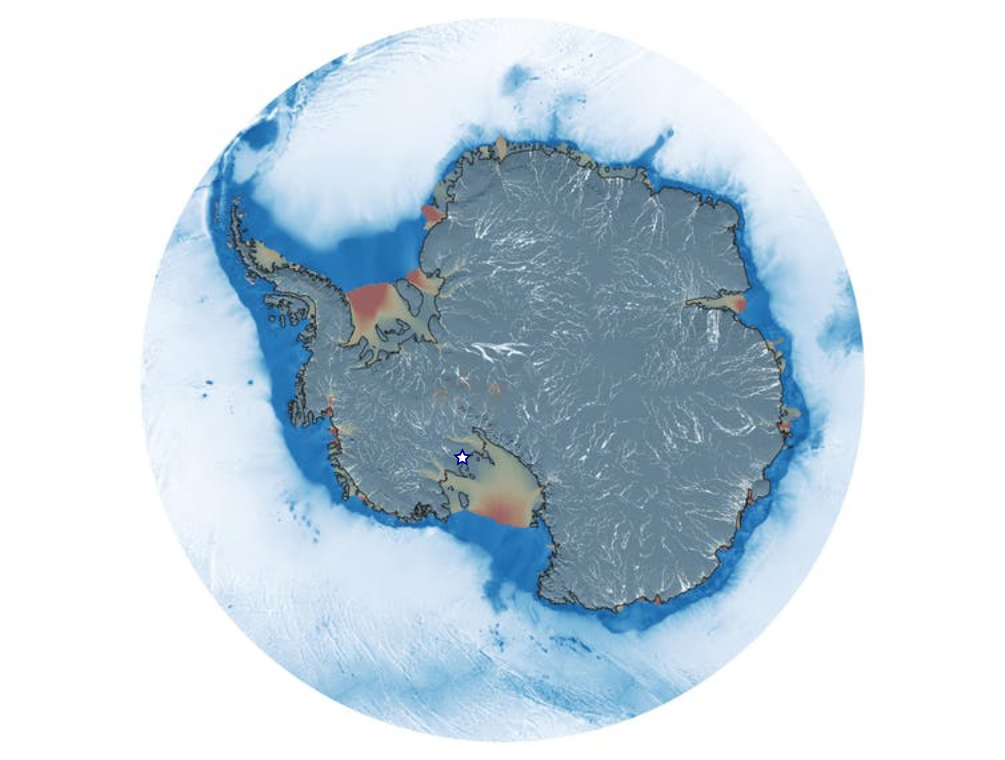
\includegraphics[width=1\textwidth]{chapters/1/antarctica.png}
\caption[Antarctica's subglacial drainage]{ Map of Antarctica with subglacial drainage routes in white \citep{le2009subglacial}, beneath Antarctica’s ice sheets in grey. Star shows study location. Warm colours denote regions of fast ice flow \citep{rignot2013ice}. Modified from \cite{horgan2022channel} }
\label{fig:antarctica}
\end{figure}  

\section{Context} \label{sec:context}

%\subsubsection{(temp)   Grounding line affects sea level}
The discharge of ice from the Antarctic Ice Sheet is accelerating, and is projected to contribute to 13--42 cm of sea level rise by the end of the century \citep{edwards2021projected}.
When ice flows off Antarctica, from sitting grounded on the continent to floating on the ocean, the volume above floatation contributes to the global sea level. The boundary between grounded and floating ice (the grounding line) is therefore an important transition. An increase in the ice flowing over the grounding line, or an inland retreat of the grounding line raises the global sea level. Processes at the grounding line, upstream in the ice sheet, and downstream in ice shelves contribute to total ice discharge \citep{rignot2011ice}. 


% In the catastrophic collapse of an ice shelf, these three aspects are thought to be linked in that the weakening or breakup of an ice shelf can cause acceleration of an ice sheet which can cause thinning and grounding line retreat.

%\subsubsection{(temp)   Upstream of the grounding line---processes}
Upstream of the grounding line, the amount of ice which flows from the centre of the ice sheet to the ocean depends on ice velocity.  In Antarctica, most ice discharge is through regions of fast flowing `ice streams', which  are characterised by low basal friction and velocities of 100s of metres per year \citep{rignot2011ice}. Slower areas where ice is stuck to the bed flow entirely via viscous deformation at velocities of 1-10s of metres per year \citep{rignot2011ice, morlighem2013inversion}.
The flow of ice is strongly forced by its coupling with the underlying bedrock \citep[e.g.][]{rose1979characteristics,engelhardt1990physical}. Changes in friction at this interface can drastically affect ice flux rates by allowing ice to slide \citep{budd1979empirical}. 
Water between ice and the bed is thought to be a fundamental factor governing changes in basal friction \citep{weertman1957sliding,iken1986combined, alley1989water}:
more subglacial water with higher pressure decouples the ice from the bed, allowing it to slide more easily. 

%\subsubsection{(temp)   Downstream of the grounding line---processes}
Downstream of the grounding line, ice shelves  are an important control on the speed of ice loss from Antarctica. Ice shelves stabilise the inland ice sheet by  providing resisting stresses which slow ice discharge at the outlets of glaciers and ice streams \citep{dupont2005assessment}. Over 80\% of ice flow off the Antarctic continent drains through floating, but fixed ice shelves \citep{pritchard2012antarctic}. When ice shelves drag past coastlines, islands, and pinning points, they generate back--stresses and buttress against ice flow \citep{dupont2005assessment, furst2016safety}.   The reduction of buttressing when an ice shelf thins or shrinks leads to the acceleration of ice loss \citep{rignot2004accelerated, berthier2012mass}, and further sea level rise. Even highly localised, concentrated thinning over a relatively small area can lead to the upstream acceleration of grounded ice \citep{reese2018far}.

%\subsubsection{(temp)   On the grounding line---processes}
Grounding line dynamics affect the Antarctic contribution to sea-level rise.  Processes at the grounding line may impact the stability of an ice sheet \citep{weertman1974stability}. Feedbacks between the grounding line and bed slope are thought to contribute to the movement of the grounding line. Ice which is floated by grounding line retreat contributes to sea level rise \citep{dowdeswell2020delicate,dupont2005assessment}. Additionally, basal melt near the grounding line is relatively strong \citep{rignot2013ice,goldberg2019accurately}. Melt near the grounding line is highly dependent on local topography \citep{rignot2013ice,goldberg2019accurately}, which can change rapidly as the grounding line moves.

%\subsubsection{(temp)   This thesis---focused on channel}
This thesis is focused on a channel incised into the base of the ice, at the intersection of ice shelf, ice stream and grounding line processes. The channel is at 152.35\textdegree E, 82.47\textdegree  S (Figure \ref{fig:antarctica}), at the grounding line of the Siple Coast, between the Kamb Ice Stream and the Ross Ice Shelf. The channel's location suggests it is coupled to both ice stream and ice shelf dynamics.
Because the channel was likely formed by melt triggered by subglacial outflow \citep{kim2016active,alley2016impacts}, better describing the formation of the channel may help to constrain the subglacial drainage system of the Kamb Ice Stream. 
Additionally, the channel likely changes the local strength of the ice shelf through localised basal melting and a change in melt patterns (as described in model channels by \cite{gladish2012ice} and \cite{sergienko2013basal}). The channel may funnel plumes of water, causing super--cooling and accretion \citep{holland2006effects}.
Lastly, the channel is probably an example of localised grounding line retreat. Due to its large size, effective pressure (defined as overburden
minus basal water pressure) is likely zero in the channel, as described by \cite{drews2015evolution}. This implies that the channel is filled with ocean water, and is part of the ice shelf cavity. The channel therefore likely forms a local embayment in the grounding line, shaped like a river mouth.


% \subsection{Outline}

In this introduction chapter, we set the context for research on the subglacial channel by reviewing the literature on sub--ice--shelf channels. Firstly, in Section \ref{sec:channels} we present an overview of ice shelf basal channels.  Next, in Section \ref{sec:ice_streams} we discuss processes upstream of the grounding line, in ice streams. In Section \ref{sec:grounding_zone_science} we outline processes at the grounding line. Section \ref{ice_shelves} covers dynamics of the ice shelf cavity, with Section  \ref{oceanography} focused on oceanography in ice shelf cavities, Section \ref{basal_melt_theory} on the theory of basal melt under ice shelves and then Section \ref{ross_ice_shelf} describing the Ross Ice Shelf specifically. Lastly, in Section \ref{sec:objectives} we outline the objectives of the research, followed by a description of the structure of this thesis (Section \ref{sec:structure})

\begin{figure}[!ht]
\centering
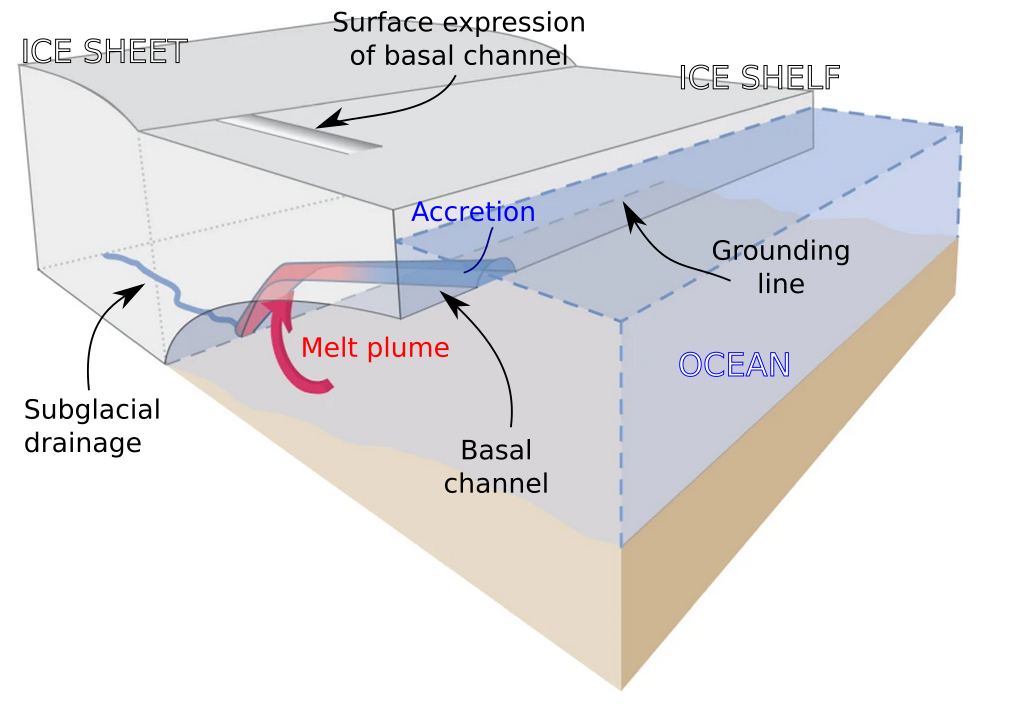
\includegraphics[width=1\textwidth]{chapters/1/chennel_schematic.png}
\caption[Channel schematic]{Schematic showing the growth of a subglacially sourced sub--ice--shelf channel. (Adapted from \cite{le2013evidence}.) }
\label{fig:channel_schematic}
\end{figure}  

\section{Channels} \label{sec:channels}

Channels incised into the base of ice shelves have been observed across Antarctica and Greenland \citep[e.g.][]{alley2016impacts,washam2019summer}. For an inventory and categorisation of ice shelf basal channels in Antarctica see \cite{alley2016impacts}.
Ice shelf channels are thought to influence basal melt of ice shelves through redistributing melt patterns \citep{millgate2013effect}. 
Increased melt rates have been observed in channels through satellite and Autonomous Phase-sensitive Radio-Echo Sounder (ApRES) based sensing techniques. For instance, \cite{marsh2016high} and \cite{stanton2013channelized} used ApRES to detect elevated melt rates ($\approx$ 20 m/yr greater) at channels on the Whillans Ice Stream and Pine Island Glacier respectively, and \cite{chartrand2020basal}  used satellite observations to find similar increased melt rates in a channel on the Getz Ice Shelf.
Modelling results from \cite{gladish2012ice} and \cite{millgate2013effect} have shown that the increase in melt rates associated with basal channels may cause a decrease in melt rates across the broader ice shelf.
However, channels are thought to generally have a destabilising effect on ice shelves, causing their structural weakening \citep{alley2019troughs}. Channels have been observed to be co-located with crevassing \citep{stanton2013channelized,alley2016impacts}, and it has been suggested that channels could speed up the collapse of ice shelves \cite{rignot2008channelized}. 

Satellite observations \citep{rignot2008recent} and modelling results  \citep{sergienko2013basal} show that ice shelf channels are generally formed in regions of high basal melt, such as the regions close to or inside grounding zones \citep{alley2016impacts}.
The majority of ice shelf channels categorised by \cite{alley2016impacts} are formed as streak lines which extend downstream of shear margins or obstructions in advecting ice.  However, some categorised channels were co--located with subglacial drainage outlets (as modelled by \cite{le2013evidence}) and were likely formed by plume melt triggered by subglacial outflow \citep{alley2016impacts}.

Drilling directly into channels in the Petermann and Pine Island Glacier respectively, \cite{rignot2008channelized} and \cite{stanton2013channelized} found buoyant plumes of melt water. Melt water plumes are thought to dominate channel circulation,  as described by modelling research by \cite{jenkins2011convection}, \cite{ sergienko2013basal} and \cite{gladish2012ice} (Figure \ref{fig:channel_schematic}). \cite{ sergienko2013basal} and \cite{gladish2012ice} suggested that the growth of channels is driven by feedbacks between the steepness of basal topography and the velocity of melt water plumes. As melt increases at the ice--ocean interface, water becomes fresher and more buoyant, causing a plume to accelerate up the ice gradient. The increase in velocity causes stronger melt as the plume entrains more salt from the deep ocean, and the melt causes a steepening and deepening of the channel such that the melt plume feedback is further stimulated \citep{sergienko2013basal}.

% Channels are thought to grow through feedbacks whereby the melting of ice produces a buoyant plume which accelerates up-slope, increasing melting and enhancing steepness of basal features \citep{sergienko2013basal}.



\section{Ice Streams} \label{sec:ice_streams}

%\subsubsection{(temp)   what are ice streams}
In Antarctica, regions of fast flowing `ice streams'  are characterised by low basal friction and velocities of 100s of metres per year. Slower areas where ice is stuck to the bed flow via viscous deformation at velocities of 1-10s of metres per year \citep{rignot2011ice, morlighem2013inversion}.
Although ice streams only make up a small fraction of the area of  Antarctica, they contribute 90\% of the total dynamical ice loss from the continent \citep{bamber2000widespread, rignot2011ice}.  Consequently, modelling their dynamics is crucial to predicting Antarctic's future ice mass budget. The high velocity of ice streams is associated with the presence of basal melt water, and deformable, saturated sediment slurries, which allow the ice to slide with little friction. This has been confirmed with seismic \citep{blankenship1986seismic, alley1987till} and radio--echo surveys \citep{robin1970radio}, borehole observations  \citep{engelhardt1997basal}, and inferences from sediment cores \citep{hodson2016physical}.
It follows that some changes in the flow of the Antarctic Ice Sheet have been attributed to changes in subglacial water distribution and drainage systems \citep[e.g.][]{alley1994water}.

%\subsubsection{(temp)   context of Antarctic subglacial drainage systems}
Despite understanding the importance of subglacial water in predicting the future of the Antarctic Ice Sheet, no model confidently describes what these waterways look like. When modelling ice flow in the Siple Coast, \cite{bougamont2015reactivation} cites subglacial drainage as a major source of uncertainty in projecting future sea level contributions.
Difficult to access beneath hundreds of metres of ice, our  knowledge of Antarctic drainage systems comes from observing paleo--ice sheet beds \citep{hattestrand1997ribbed, lewis2006age}, remote sensing \citep{schroeder2013evidence}, inverse modelling \citep{morlighem2013inversion} and sparse borehole drilling \citep{engelhardt1997basal}.
Bed conditions such as intermittent pools of water or saturated
sediments, lakes, channelisation of water, and areas with frozen beds with no drainage system have all been found to be widespread \citep{carter2009using, schroeder2013evidence, young2016distribution}. 

%\subsubsection{(temp)   theorys of subglacial drainage in Antarctica}
Current  models of subglacial  drainage in Antarctica are based on theories of alpine glacier  drainage, as alpine glaciers are generally easier to study due to their accessibility, size, and seasonal change. However, ice stream drainage systems are thought to be different from those in mountain glaciers, in that they are characterised by smaller hydraulic gradients, less water supply, thicker ice and softer bed substrate.
To encapsulate varied and often unknown drainage conditions, all large scale models of subglacial drainage in Antarctica have assumed that areas of sliding have sheet or porous flow \citep{flowers2015modelling}. This is a broad assumption that aims to approximate bed conditions and is normally based on two findings: Firstly, \citet{alley1989water} predicted that if there was no channelised flow, sheet flow would dominate drainage systems under ice sheets. Later, \citet{alley1996towards} showed that in the absence of information about basal conditions, modelling drainage as sheet flow is a reasonable approximation for a wide variety of bed conditions. The \citet{alley1996towards} pure sheet flow model can reasonably accurately describe relationships between basal shear stress and water pressure but is too simple to show changes in the subglacial drainage systems, which are believed to exist \citep[e.g.][]{schroeder2013evidence}.

Canals (channels incised into the bed substrate) are thought to be the most representative model for `discrete' drainage elements in Antarctica \citep[e.g.][]{walder1994channelized,simkins2017anatomy}. Discrete drainage elements like canals or channels are confined to certain routes, and contrast with drainage elements like porous or sheet flow which are modelled across the entire ice base. Compared to other drainage models, the theory of subglacial canals is least developed. Active canals have not been observed, and the models which summarise the erosion dynamics which govern the width of canals have not been robustly compared against observations \citep[e.g.][]{damsgaard2017sediment}. As opposed to R--channels, (channels incised into the ice base) canals are thought to exist at a low effective pressure (defined as overburden
minus basal water pressure) \citep{walder1994channelized}. Model canals support a relationship with subglacial water pressure increasing as discharge increases \citep{walder1994channelized,ng1998mathematical}, whereas R--channels support the opposite  \citep{rothlisberger1972water,shreve1972movement}. 
It is believed that a positive relationship between discharge and water pressure is a requirement for the feedbacks that drive ice streams, whereby low effective pressures (high water pressure) and fast sliding lead to more frictional melt \citep{fowler1996ice}.
R--channels, because they tend to 
increase effective pressure as discharge is increased, favour slow ice flow. 
Additionally, it is not clear that the low hydraulic gradients and low melt rates under Antarctica are sufficient to support persistent R--channels; though R--channels have been argued to exist at the outlets of draining lakes \citep{evatt2006subglacial,pattyn2008investigating}, as well as under the shear margins of ice streams, where there are high melt rates \citep{perol2011control}. 

%\subsubsection{(temp)   observations of subglacial water in Antarctica}
Most observations of subglacial water in Antarctica are related to documenting the existence of subglacial lakes \citep[e.g.][]{carter2007radar,wright2012fourth,siegfried2018thirteen}.
Airborne radar surveys first revealed subglacial lakes in the 70s \citep{robin1970radio}. Since then over 400 subglacial lakes have been found \citep{siegert2016recent} with radar--echo sounding reflections \cite[e.g.][]{carter2007radar} or through repeated altimetry that shows localised drops or uplifting in the ice surface that are the result of lakes draining or filling \citep{wingham2006rapid, stearns2008increased, gray2005evidence, fricker2007active}. 
Other drainage features have been observed in paleo ice sheet beds, now underwater  \cite[e.g.][]{nitsche2013paleo, anderson2008geomorphology}. These identify large channels which are hypothesised to be formed from subglacial melt water due to the fact they are parallel to flow or are anastomosing.  Using radar in an area of the Antarctic Ice Sheet, \cite{schroeder2013evidence} found what they believe is a transition from channelised drainage system to a distributed drainage system by observing changes in specularity of a radar reflection. However, the only imaging of active Antarctic subglacial drainage channels comes from \cite{drews2017actively}, who imaged a subglacial channel near a grounding line. \cite{drews2017actively} hypothesise that the channel has formed a large esker, and note that with consistently low effective pressures near a flat grounding line R--channels will grow large.

\subsection{Kamb Ice Stream}

%\subsubsection{(temp)   variability of the kamb}
The  Kamb Ice Stream  once  drained  the  interior  of  the  West  Antarctic  Ice  Sheet  to  the Ross Ice Shelf, flowing faster than $350$ $\mbox{m/yr}$ \citep{ng2004fast}.  Around $150$ years ago, it stagnated to a speed of around $10$ $\mbox{m/yr}$ \citep{ng2004fast}.   As  a  result  of  this  change  in  flow,  the  Kamb Ice Stream is  often referenced as an example of internal variability in ice stream flow \citep[e.g.][]{hulbe2004west}.  
The grounding line of the Kamb ice stream is thought to have occupied its current position for around 150 years, prior to which it was downstream \citep{fried2014grounding}. \cite{horgan2017poststagnation} suggest that after the stagnation of the Kamb Ice Stream the grounding line likely retreated to its current location.
If the Kamb Ice Stream reactivated, ice discharge would potentially increase by 20 Gt/a \citep{jacobel2009spatial}. 
% If another ice stream were to shut down, discharge from Antarctica would decrease by a large amount. 
While variability in the flow of the Kamb Ice Stream is attributed to changes in subglacial drainage, there is no clear evidence of how this happened. The leading hypothesis proposes that water was rerouted  away  from  the  ice  stream  leaving  its  base  dry \citep[e.g.][]{anandakrishnan1997stagnation}, though observations of water at the base of the ice stream contradict this hypothesis \citep{engelhardt1997basal}.  A second hypothesis for the slowdown describes changes in the shape of subglacial networks, from an inefficient high--pressure system that fosters sliding to an efficient, low--pressure system that doesn’t greatly reduce bed friction \citep{lelandais2018modelled,retzlaff1993timing}. Other models describe ice stream variability as driven by changes in the thermal regime at the bed, between frozen/stuck and wet/sliding regimes \cite[e.g.]{robel2013dynamics}.

%\subsubsection{(temp)   kamb subglacial drainage}
The subglacial drainage system (water) of the Kamb Ice Stream was modelled by \cite{le2013evidence}. While the water flow rates in this model have high uncertainties, the estimated flow routing was mapped directly from relatively accurate pressure gradients based on ice thickness maps. \cite{le2013evidence} founds a valley in the hydro--potential field, and predicted the confluence of almost all subglacial drainage. \cite{kim2016active} suggested that there is likely channelised drainage under the Kamb Ice Stream, through finding linked subglacial lakes whereby the flooding of one lake fills downstream lakes.  The predicted flow path and potential channelised drainage route meets the grounding line at a large channel feature which is the subject of this thesis. 


\newpage
\section{The grounding zone} \label{sec:grounding_zone_science}


\begin{figure}[!ht]
\centering
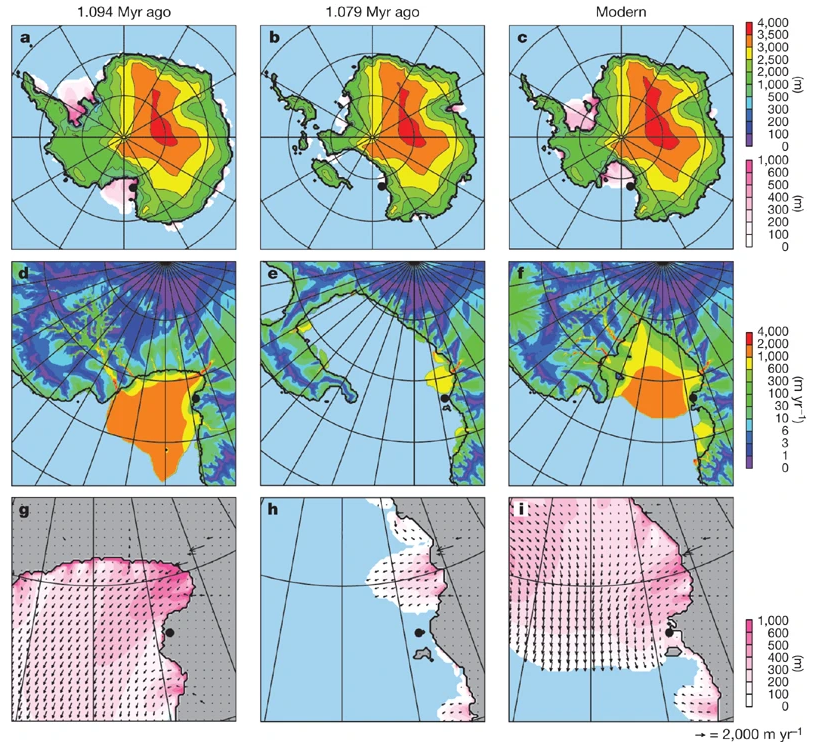
\includegraphics[width=1\textwidth]{chapters/1/pollard.png}
\caption[Modelled past Ross Ice Shelf extent]{From \cite{pollard2009modelling}.
Grounded ice elevations and floating ice thicknesse from a) 1.094 Myr ago, b) 1.079yr ago (MIS 31 retreat) and c) present day.
Surface ice speeds (m/yr), from higher-resolution (10 km) nested runs over the Ross embayment for d) 1.094 Myr ago, e) 1.079yr ago and f) present day.
Floating ice thicknesses (m) and velocity vectors from the nested simulations, enlarged over the western Ross embayment for  g) 1.094 Myr ago, h) 1.079yr ago and i) present day.
The location of the AND-1B drill location is shown by the black dot.}
\label{fig:pollard}
\end{figure}  

% \subsection{Tidal pumping, estuaries}
% % https://tc.copernicus.org/articles/15/1863/2021/tc-15-1863-2021.pdf
The `grounding line/zone' is the boundary between grounded and floating ice. For larger scale processes, this boundary is often simplified as a line \citep[e.g][]{gudmundsson2013ice}, though in reality the boundary spans an inter-tidal area \citep[e.g][]{christianson2016basal}, termed the grounding zone. Around the grounding zone, the interaction of the ocean and ice sheet base affects ice sheet flow and basal melt.
There are numerous observations of ice streams which accelerate and decelerate depending on the tide \cite[e.g.][]{winberry2009basal,anandakrishnan2003ice}. 
When an ice shelf rises and falls with tidal cycles, ice bends at the grounding line. Various modelling approaches agree that tidal bending has the potential to move water and that with each tidal cycle, the ocean extent changes  \citep{sayag2013elastic,walker2013ice}. 
For this reason, the grounding line is commonly termed the grounding zone. Observations confirm that the transition from grounded to floating ice occurs over some distance \cite[e.g.][]{brunt2019assessment}, and that the transition from fresh water basal hydrology to salt is not clear cut \cite[e.g.][]{christianson2016basal}.
Ice sheet models are highly sensitive to basal melt at the grounding line, and models show that an increase in basal melt enhanced by the inland intrusion of salt water can cause a large change in the forecast volume of an ice sheet \citep{robel2022layered}.


\subsection{West Antarctic Ice Shelf instability}

%\subsubsection{(temp)   grounding line controls ice sheet dynamics}

In contextualising paleo ice sheet extent \cite[e.g][]{naish2009obliquity,pollard2009modelling}, grounding line location is used as a proxy for the size of an ice sheet. Grounding line location and dynamics are chronicled to identify the past collapse of the ice sheet. 
The modelled paleo extent of the Ross Ice Shelf and West Antarctic Ice Sheet, 1.094 million years ago, is shown in Figure \ref{fig:pollard}.

%\subsubsection{(temp)   marine ice sheet wont regrow}
The West Antarctic Ice Sheet is a marine ice sheet, meaning it is largely grounded below sea level \citep{fretwell2013bedmap2}. This is unstable in that if it were to collapse (as in Figure \ref{fig:pollard} b), it would not grow back in modern climate conditions \citep{oerlemans2021analytical}. In the present day, snow fall augments ice mass and is balanced by the discharge of ice, which flows from the interior of the continent to the sea \citep{rignot2002mass,paterson2016physics}. However, if the ice sheet were to collapse, snow would fall on the ocean, and would not augment ice mass. The formation of a marine ice sheet relies on lower sea levels with enough landmass to sustain  a positive mass balance \citep{oerlemans2021analytical}. 



% Both stable grounding line locations and runaway retreat have been observed  where?how?what? \citep{yokoyama2016widespread}.


%\subsubsection{(temp)   Marine instability }
The West Antarctic Ice Sheet has retreated quickly in the past \citep{yokoyama2016widespread}. This observation, along with theoretical ideas of instabilities in marine ice sheets \citep[e.g.][]{katz2010stability} has led to a hypothesis that the West Antarctic Ice Sheet could collapse quickly in the future \citep{vaughan2008west}.
The most heavily cited mechanism for describing this collapse is the marine ice sheet instability \citep{weertman1974stability}. The marine ice sheet instability postulates that with no change in accumulation, a reverse bedslope is an unstable grounding line position, while a positive bedslope is stable. This instability theoretically applies to a one dimensional glacier, which is thought to be representative of a glacier with no lateral bounds.  If the grounding line retreats on a reverse bed slope, ice thickness increases, which leads to faster ice discharge and  further retreat.  Stability is only achieved when the downstream flux gradient at the grounding line exceeds the accumulation rate \citep{haseloff2018effect}. On a reverse slope, a perturbed grounding line will advance or retreat until the grounding line reaches a location with a positive slope. 

%\subsubsection{(temp)   Rebutting the marine ice instability}
While the marine ice sheet instability is widely cited as a source of concern, with more realistic models \cite{haseloff2018effect}, \cite{gudmundsson2013ice} and \cite{jamieson2012ice} all found that marine ice sheets confined laterally or by ice shelves are not necessarily unstable on reverse bed slopes. They found that buttressing can restore stability to marine ice sheets with reverse bed slopes, and that the marine ice-sheet instability may not apply to marine ice sheets with lateral and/or ice shelf buttressing \citep{haseloff2018effect}. It follows that is not clear to what extent the West Antarctic Ice Sheet is  unstable \citep{vaughan2008west}. Some areas of the West Antarctic Ice Sheet like Thwaites Glacier and Pine Island Glacier appear to be collapsing due to a combination of the marine ice sheet instability and the southward intrusion of relatively warm currents of Circumpolar Deep Water \citep{ favier2014retreat, joughin2014marine}. Other areas, such as the Siple Coast, appear to be presently stable \citep{hindmarsh1996stability}, and have retreated relatively slowly in the past \citep{conway1999past}.




\section{Ice Shelf Cavity} \label{ice_shelves}

\subsection{Oceanography} \label{oceanography}
% https://eos.org/science-updates/exploring-the-unknown-of-the-ross-sea-in-sea-ice-free-conditions

\begin{figure}[!ht]
\centering
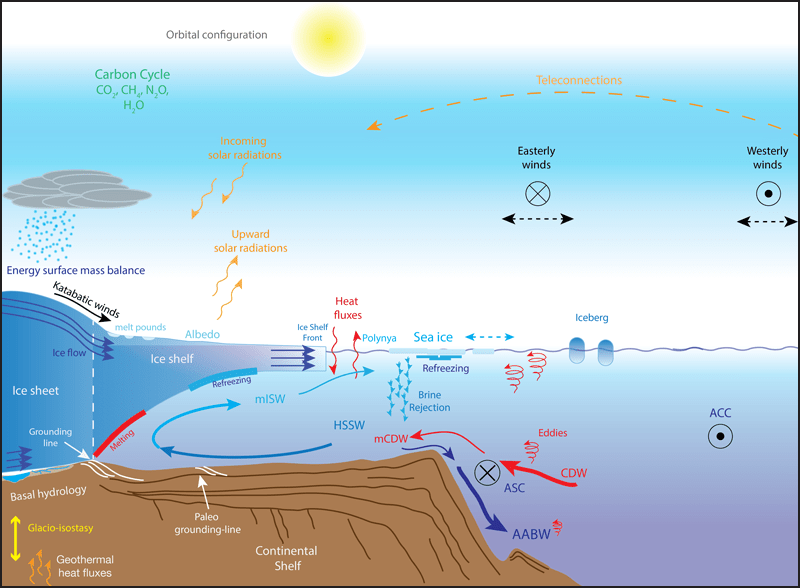
\includegraphics[width=1\textwidth]{chapters/1/ocean_schematic.png}
\caption[Ross Ice Shelf circulation schematic]{ Two dimension schematic showing dominant ocean processes linked to the Ross Ice Shelf. Acronyms represent water masses. A circled X means flow into the image, and a circled dot means flow out of the image.  Reproduced with permission from \cite{santis2018ross}. }
\label{fig:ocean_schematic}
\end{figure}  

%\subsubsection{(temp)   Ice shelves connect ice sheets to oceans}
Floating ice shelves which fringe Antarctica provide a direct connection between the world's oceans and the Antarctic Ice Sheet. The coupling between these two important entities can be reduced to processes which occur at the interface between ice shelves and the ocean \cite{holland2003modelling}. These processes have large impacts on both the ice sheet and the ocean. As climate change warms the oceans, the heat melts ice shelves which thin and weaken, reducing their restraint on the flow of the ice sheet \citep{pritchard2012antarctic}. Based on climate projections for the twenty-first-century, heating of the oceans is predicted to increase mass loss of Antarctica's ice shelves by between 41\% and 129\% \citep{naughten2018future}. Conversely, as ice shelves melt they release large quantities of fresh cool water into the ocean \citep[e.g.][]{holland2006effects}. This water has a strong effect on the production of sea ice \citep{langhorne2015observed}, and is one of the building blocks of the Antarctic Bottom Water which fills the worlds deep oceans \citep{foldvik2004ice}.

%\subsubsection{(temp)   Southern Ocean oceanography}
The Southern Ocean is unimpeded by obstacles for its entire 360 degree span around Antarctica, allowing the free flow of wind and seas. The strong westerlies present drive the worlds strongest current, the Antarctic Circumpolar Current which transports a mean 100-150 million $\mathrm{m}^3$/s \citep{knauss2016introduction} (Figure \ref{fig:ocean_schematic}, ACC). The Antarctic Circumpolar Current connects to the Atlantic, Pacific, and Indian Oceans, and propels portions of the principal currents in each ocean, as well as acting as an intersection (a large round--about) for exchange between them \citep{knauss2016introduction}. The circumpolar current dominates the Southern Ocean, blocking direct north--south transfer, and driving movement of the relatively warm and salty water mass, named Circumpolar Deep Water, eastward and in places southward \citep{knauss2016introduction}. Some ice shelves, such as those of the Pine Island and Thwaites Glaciers \citep{nakayama2019pathways} in the Amundsen and Bellingshausen Seas,  are strongly affected by this warm water which transports heat and salt south \citep{nakayama2018origin}, increasing basal ice shelf melt. 

%\subsubsection{(temp)   Mode 1 ice shelf circulation}
Basal melt is driven by the circulation of water under ice shelves, which transports heat and salt from the open ocean to the ice base (Figure {\ref{fig:ocean_schematic}}. The largest circulation pattern in ice shelf cavities starts in the open ocean surrounding Antarctica \citep{jacobs1979circulation}. Sea ice proliferates on the open ocean, growing from a mean summer extent of 3.1 million $\mathrm{km}^2$ to a mean winter extent of 18.5 million $\mathrm{km}^2$  \citep{hobbs2016review}. As sea ice freezes, it leaches brine (Figure {\ref{fig:ocean_schematic}}, Sea Ice, Refreezing, Brine Rejection). Brine is relatively dense and so sinks, forming the water mass known as High Salinity Shelf Water (Figure {\ref{fig:ocean_schematic}}, HSSW). The dense High Salinity Shelf Water flows inland along the sea floor until it meets ice at the grounding line \citep{jacobs1979circulation}. There, the availability of salt causes melting of the ice base, releasing fresh water (Figure {\ref{fig:ocean_schematic}}, Melting). The buoyant melt water forms a plume which rises up the gradient of the ice shelf (Figure {\ref{fig:ocean_schematic}
}, mISW). The plume entrains salty water from the depths of the ocean to mix with the ice boundary layer and melts the ice base \citep{jacobs1979circulation}. 
This process is thought to be the dominant source of vertical mixing under ice shelves, essential for the transport of salt through the stable water column from the bottom of the ice shelf cavity to the ice base.  
A positive feedback between momentum of the plume and melt drives this process. Momentum enhances the entrainment of salt and heat, causing melt which results in a gain in buoyancy, allowing the plume to accelerate up a positively sloped ice base  \citep{jenkins1991one}.  The plume continues to ascend away from deep salty waters. 

%\subsubsection{(temp)   Accretion}
Eventually, entrainment wanes until the plume lacks salt and heat. The plume ceases to melt the ice, but residual momentum and buoyancy propel the plume. The pressure and freezing point of ascending water drops, causing the plume to dip below the freezing point, becoming super--cooled \citep{holland2006effects}.  Super--cooling is slowed by the growth of frazil ice, small ice crystals suspended in the water column. Eventually, the plume reaches equilibrium height and detaches from the sloped ice base, plateauing into the ice cavity at a constant depth  \citep{hewitt2020subglacial}. 
The crystals of frazil formed from the super--cooling of water are thought to eventually consolidate at the ice base, forming layers of marine ice \cite[e.g.][]{fricker2001distribution} (Figure {\ref{fig:ocean_schematic}
} Refreezing).  Over time this layer is thought to metamorphose and consolidate, first forming  a platelet layer, then continuing to become less porous \citep{craven2009properties}. Marine ice is distinct from glacial (meteoric) ice in that it is salty. While accretion may also occur directly on the ice base, some observations \citep{vavnkova2021nature} and modelling \citep{bombosch1995modeling} suggest marine ice forms from the deposition of frazil.  Accumulation of marine ice or accretion occurs mainly away from the edges of ice shelves. 

%\subsubsection{(temp)   Ice pump process}
% While most global ocean circulation is driven by momentum from the wind and tides, ice shelf cavities are uniquely disconnected from the ocean. 
The dominant circulation pattern in an ice shelf cavity (described above) is driven by density changes through melting and freezing which cause water masses to change salinity \citep{jacobs1979circulation}. Ice melt causes both cooling and freshening of water, which have opposite effects on the density of water (and in reverse for formation of sea ice). However, the change in salinity has a greater effect on density, so melt water is buoyant \citep{jenkins1991one}. The circulation pattern described causes a net transfer of ice and energy in two steps. Firstly, the formation of sea ice on the open ocean effectively drives the removal of ice from the ice shelf. Secondly, ice shelf melt near the grounding line drives the formation of marine ice under an ice shelf.
The second part of this process is known as the `ice pump' described by \cite{lewis1986ice}. Following this reasoning, the first part is effectively a `negative ice pump', as negative potential ice through high salinity water is transported rather than potential ice through relatively fresh water.
These processes are visible in satellite observations which confirm a pattern of negative basal mass balance around the perimeter of ice shelves, and positive or zero basal mass balance at the centre \citep[e.g.][]{rignot2013ice}. 



%\subsubsection{(temp)   Channels}
Additional to these broad distributions of basal melt across ice shelves 10s to hundreds of kilometres wide, large changes in basal melt can be found over spatial scales of hundreds of metres \citep[e.g.][]{marsh2016high,stanton2013channelized,stewart2019basal}, which are likely caused by localised circulation \citep{sergienko2013regular}. Local variability is particularly visible near the grounding line, for example at topographical features like ice shelf channels, which have been identified as some of the strongest regions of ice shelf melt away from the open ocean \citep[e.g.][]{marsh2016high, stanton2013channelized}. 
Through feedbacks with basal topography \citep{sergienko2013regular},  channels stimulate the growth of meltwater plumes. These plumes, driven by buoyancy are an important source of vertical mixing, which transports salt and heat from the ocean bottom to the ice shelf base \citep{macayeal1984thermohaline}.



%\subsubsection{(temp)   Tidal vertical mixing}
Vertical mixing is also enhanced by tidal currents \citep{macayeal1984thermohaline}.  Horizontal tidal currents experience friction on boundaries with the sea floor and ice base. The friction induces shear and turbulence, causing the development of mixed layers at both boundaries. In shallow areas tidal currents are stronger, creating  thicker mixed layers which provide greater vertical transport  \citep{makinson2002modeling}. If the cavity is shallow enough, the top and bottom mixed layers meet and vertical transport is not restricted by a stable middle layer.

%\subsubsection{(temp)   Coriolis effect}
The broad theoretical model of ice shelf overturning, as pictured in Figure \ref{fig:ocean_schematic}, describes vertical and N-S circulation though neglects the complexity of 3D circulation \citep{holland2006effects}. In reality, earth's rotation causes austral currents to deflect left, generally resulting in stronger outflow on the western sides of Antarctic ice shelves. As a result, buoyant plumes do not flow up--gradient unless they are constrained by topography. Due to the low-friction of the ice shelf base, plumes are almost geostrophic and are found to contour around ice shelves \citep{jenkins2016simple}. The geostrophic balance is between the Coriolis force and buoyancy force, which is deflected up--gradient by the ice base. Currents follow iso-baths and horizontal movement of water dominates ocean flow. As a result, currents will not rise and become super--cooled under a smooth ice base, topographic roughness or constraints are necessary to force up--welling \citep{holland2006effects}.

%\subsubsection{(temp)   impact of ISW}
Up--welling forms cool melt water which flows out of the ice shelf cavity and has a strong impact on global oceans. This very cold water mass, named Ice Shelf Water (Figure {\ref{fig:ocean_schematic}
}, mISW),  mixes with other water masses to form Antarctic Bottom Water (Figure {\ref{fig:ocean_schematic}
}, AABW). Antarctic Bottom Water is a super--dense water mass which sinks and spills off the Antarctic continental slope, spreading northward to fill most of the depths ($>$4 km) of the worlds oceans \citep{orsi1999circulation}. 
Additionally, Ice Shelf Water which reaches the open ocean surface is relatively cold and fresh and often filled with frazil ice, both of which enhance sea ice thickening \citep{langhorne2015observed}.
Climate models are particularly sensitive to the outflow of Ice Shelf Water. Modelling results suggest that increases in melt water can increase sea ice extent and affect the global climate \citep[e.g][]{merino2018impact,golledge2019global,bronselaer2018change}, though the treatment of ice shelf melt water flux in these models is not yet realistic \citep{jourdain2020protocol}.

\subsection{Basal melt theory} \label{basal_melt_theory}

%\subsubsection{(temp)   melt v dissolving}
What is generally called `melt' can be driven by the supply of heat or salt to the ice base \citep{wells2011melting}. When heat is supplied to the ice base, melting occurs when the ice base is warmed to the freezing point of fresh water. However, `melt' can also occur with ice below the freezing point of fresh water when salt is transported to the ice base. In this case, the salt locally lowers the salinity--dependent freezing point, allowing ice to change to liquid phase \citep[e.g.][]{mcphee1987dynamics}. Strictly, this is the `dissolving' of ice \citep[e.g][]{malyarenko2020synthesis}, whereby the amount of ice ablated is dependent on the quantity of salt transported to the ice base.
Basal ice shelf melt is often driven by salt supply. For example, near the grounding line of the Ross Ice Shelf, 510 m below sea level, \cite{robinson2020ice} found sea water was at -2.25 \textdegree C and 34.75 psu and predicted melt rates of 0.2 m/yr, which were confirmed independently by observations. This melt falls under the dissolution regime as it is occurring at temperatures beneath the freezing point of fresh water.

%\subsubsection{(temp)   boundary layers}
% Basal melt is driven by the transport of heat and salt to the ice shelf base \citep{holland1999modeling}. 
As described above, transport of heat and salt to the ice shelf base occurs on a  larger ($>$km) scale from the open ocean to the ice shelf cavity \citep{holland1999modeling}. Additionally, the fine scale ($<$m) is important for melt rates. Salt and heat must be in physical contact with the ice boundary to cause melt \citep[e.g.][]{jenkins2010observation}. 
Melt of a horizontal ice--ocean interface has a stabilising effect on the ocean cavity. Melt contributes to a low density layer at the top of the water column. This isolates the ice boundary from the warmer saltier sea below. At the ice--ocean interface, shear currents driven by buoyancy, pressure gradients or tides produce turbulence, causing mixing and vertical transport of heat and salt to the ice boundary. When modelling melt, the ocean boundary layer adjacent to the ice shelf is generally divided into three sublayers: The inter-facial sub-layer, millimetres to centimetres from the ice boundary, characterised by the fact that transfer of momentum is driven by molecular viscosity and direct interaction with the roughness of ice \citep{jenkins2010observation}. 
The surface layer, metres from the ice boundary, where turbulent mixing is influenced by the boundary. The outer layer, 10s of metres from the boundary, where turbulence is unaffected by the boundary and mixing is determined mainly by Ekman transport and stratification. Observations of these boundary layers and turbulent processes exist \citep[e.g.][]{jenkins2010observation,davis2019turbulence}, though they are very sparse and so processes are generally poorly parametrised \citep[e.g.][]{jenkins2010observation,malyarenko2020synthesis}.
 

\newpage
\subsection{Ross Ice Shelf} \label{ross_ice_shelf}

\begin{figure}[!ht]
\centering
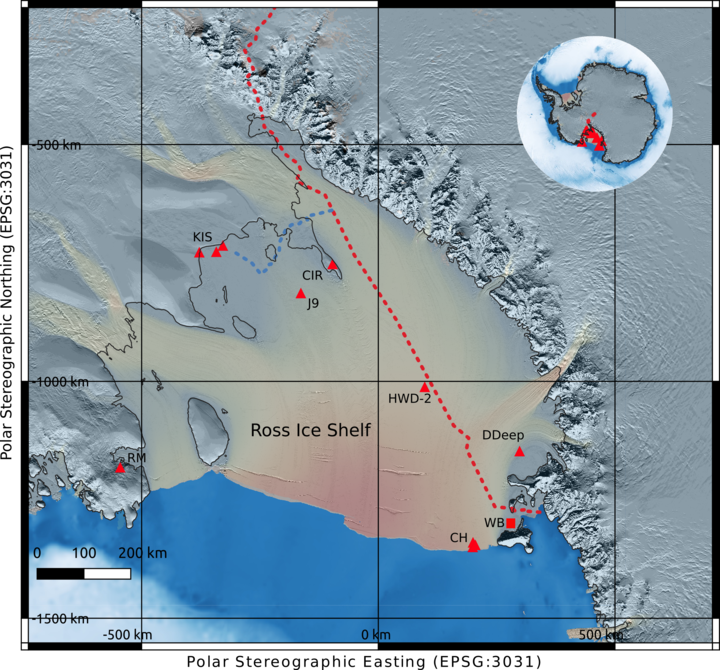
\includegraphics[width=1\textwidth]{chapters/1/ris.png}
\caption[Ross Ice Shelf map]{Map showing the Ross Ice Shelf. Background image is REMA 100m Mosaic \citep{howat2019reference}  overlaid with MEaSUREs Phase-based Ice Velocity \cite{rignot2011ice}. Red triangles mark the locations of boreholes through the Ross Ice Shelf labelled with the borehole name. KIS is the Kamb Ice Stream. This field location focused on in this thesis is at the left red triangle under the KIS label. Red dotted line shows the South Pole Traverse Route. Blue dotted line shows the traverse to KIS.}
\label{fig:ris}
\end{figure}  

The Ross Ice Shelf is the world's greatest ice drainage basin, with around 130 Gt ice/yr discharged through the shelf \citep{rignot2008recent} (Figure \ref{fig:ris}). Spanning around 400,000 $\mathrm{km}^2$, the Ross Ice Shelf is fed by the ice streams of the Siple Coast to the south east, which discharge ice from the West Antarctic Ice Sheet, and glaciers of the Transantarctic Mountains to the west, which drain from the East Antarctic Ice Sheet. 

%\subsubsection{(temp)   Range of basal mass balance}
The Ross Ice Shelf loses around 50 Gt/yr of ice through basal melt \citep{rignot2013ice,moholdt2014basal,das2020multidecadal}.  Basal melt rates  average around 12 mm/yr \citep{moholdt2014basal}. Point melt rates have been observed as high as 50 m/yr at the ice front \citep{stewart2019basal}, and up to 20 m/yr at localised channel features near the grounding line \citep{marsh2016high}. Unlike the Amery Ice Shelf where 100s of metres of marine ice have been found \citep{craven2009properties}, no more than 6 m of marine-ice accumulation has been found underneath Ross Ice Shelf \citep{zotikov1980core}, although no comprehensive survey exists.

%\subsubsection{(temp)   sub--ice--shelf ocean circulation}
There are few observations of circulation under the ice shelf \citep[e.g.][]{jacobs1979circulation,stewart2018ice,stevens2020ocean,robinson2020ice}, shown in Figure \ref{fig:ris}.
Of these campaigns, \cite{jacobs1979circulation} and \cite{stevens2020ocean}  profiled ocean structure in the central Ross Ice Shelf. At both sites, the basal accretion of crystals was observed. Additionally, both found a mid-column with features which increase fluxes of heat and salt, such as interleaving, intrusion, and overturns  \citep{stevens2020ocean}. In general, the two sites had large differences in ocean structure, for instance, \cite{stevens2020ocean} found generally greater salinity and additional to the three layers observed by \cite{jacobs1979circulation} who found a 30 metre thick basal melt layer. These large differences may be due to the fact the two locations were separated by different circulation cells which divide regions of the cavity, as suggested by simulations of the cavity \citep{pritchard2012antarctic}.
Observations at the ice front \citep[e.g.][]{smethie2005circulation} and physical simulations of ocean circulation in the cavity by \cite{holland2003ice} provide a broad picture of flow in and out of the cavity. Salty warm water flows into the cavity at the western third of the ice shelf, and cool fresh water flows out in the centre. This is a generalisation, finer scale observations reveal more complex dynamics, for example, \cite{robinson2014evolution} found cool fresh outflow on the Western flank of the cavity. 
Within the Ross Ice Shelf cavity, the tidal range is predicted to be greatest on the Siple Coast \citep{padman2003tides}. There, the peak to peak tidal range is around 3 m. Typical tidal currents are predicted to be around 5 cm/s under the ice shelf \citep{padman2003tides}.

%\subsubsection{(temp)   Stability - ocean induced}
The stability of the Ross Ice Shelf is partially dependent on its coupling with the warming ocean. Some heat supplied to the ice shelf cavity originates from the Circumpolar Deep Water \cite[e.g.][]{rignot2002mass}. This water mass intrudes across the Ross Sea Break along troughs in the sea floor, becoming mixed with other water masses before flowing under the ice shelf \citep{castagno2017temporal}. Relative to ice shelves of the Amundsen sea or the Antarctic peninsula, which are thought to be susceptible to break up from the intrusion of warm Circumpolar Deep Water \citep{ favier2014retreat}, the Ross Ice Shelf is less well connected to the warmer saltier waters to the north \citep{dinniman2011model}. In the Ross Sea, the Circumpolar Deep Water is not only cooler initially and travels a longer distance to reach the ice shelf, but it also experiences more vertical mixing with surface waters. This dissipates the heat available to be advected under the ice shelves \citep{dinniman2011model}.

%\subsubsection{(temp)   ice stability , Modern ice source}
The Ross Ice Shelf is currently stable \citep{paolo2015volume}.  Its present extent repeatedly arises in model experiments simulating Antarctica's past \citep{pollard2009modelling}, suggesting that its current configuration is stabilised by bedrock topography such as the pinning points of the Ross and Roosevelt Islands. Surface textures on the Ross Ice Shelf like flow stripes and crevasses record the provenance of modern ice. Analysis of these textures reveals that ice flux through the Transantarctic Mountains has been relatively stable for at least 500 years, while ice supply from individual ice streams has stagnated and reactivated over century timescales \citep{hulbe2007century}. Flow lines suggest that about 850 years ago Whillans Ice Stream stagnated, then reactivated 400 years later. Similarly, the MacAyeal Ice Stream stagnated and reactivated around 800-650 years ago, and the Kamb ice stream stagnated around 150 years ago \citep{hulbe2007century}.
% These ice streams feed the Ross Ice Shelf from the West Antarctic Ice Sheet \citep{hulbe2007century}. 

%\subsubsection{(temp)   Historic RIS extent}
The stability of the Ross Ice Shelf and the stability of the West Antarctic Ice Sheet are thought to be closely linked. While the Ross Ice Shelf buttresses flow from the West Antarctic Ice Sheet, the West Antarctic Ice Sheet feeds the Ross Ice Shelf. In the past, the West Antarctic Ice Sheet has rapidly disintegrated in sync with the collapse of the Ross Ice Shelf \citep{pollard2009modelling}. 
Sediment cores  show that over the past 5 million years the location of the present Ross Ice Shelf front has fluctuated between ice shelf, ice sheet and open ocean \citep{naish2009obliquity}. This implies that both the ice shelf and the ice sheet advanced and retreated.
Modelling experiments by \cite{pollard2009modelling} extrapolated from the \cite{naish2009obliquity} data suggest that the entire West Antarctic Ice Sheet repeatedly expanded and collapsed over the last 5 million years.
At the Last Glacial Maximum ($\approx$20 kyr before present) grounding lines advanced to the continental--shelf edges, 300 km north of Ross Island  \citep{mckay2008retreat} .
Beginning around 5000 years ago, the ice shelf suffered a widescale collapse  on the continental shelf. This was followed by continuous grounding line retreat until the current ice shelf and ice sheet extent was reached aroun 1500 years ago \citep{yokoyama2016widespread}. 
Predictions for the future of the Ross Ice Shelf and West Antarctica show large differences in ice sheet sensitivity to climate forcing because of differences in model parameterisations \citep{deconto2016contribution,golledge2015multi,edwards2021projected}.

\section{This Thesis}
% \subsection{Context - Detail what is known about the channel from before}

This thesis is focused on a basal channel at the grounding line where the Kamb Ice Stream meets the Ross Ice Shelf. The channel has been noted previously in literature \citep{le2009subglacial,alley2016impacts,kim2016active,goeller2015subglacial,horgan2017poststagnation}, and was profiled by airborne radar as part of the Center for Remote Sensing of Ice Sheets (CReSIS) airborne radar project \citep{arnold2020cresis}. The channel is migrating upstream at around 1-1.5 m/yr and shows present surface lowering \citep{kim2016active}. While \cite{kim2016active} suggested that the formation of the channel coincides with the ice stream shutdown,   \cite{horgan2017poststagnation} suggests that the grounding line retreated to its current location after the shut down. Because the channel is at the outlet of an inferred subglacial drainage system, \cite{le2009subglacial}, \cite{alley2016impacts} and \cite{kim2016active} suggest that the channel is subglacially sourced. This implies that channel growth was triggered by subglacial outflow. The channel does not appear to be a relic streak line formed by the advection of ice past an obstruction, as the channel is not a linear feature but appears to meander downstream.


%\subsubsection{(temp) Opportunities}

The channel provides an opportunity to study ice--ocean interaction at the intersection of the ice stream and ice shelf and the grounding line.  Constraining a description of the channel and processes associated with the channel and its formation may help to explain and model a variety of important processes upstream and downstream from the channel. Firstly, better quantifying subglacial outflow at the channel may help to constrain Kamb's subglacial drainage system, which has been cited as a major source of uncertainty in projecting future sea level contributions \citep{bougamont2015reactivation}. Secondly, better constraining the processes involved in inland migration of the channel, and the cause of stability or retreat may help to predict future grounding line retreat on the Siple Coast. Lastly, better understanding interaction between the ocean and ice shelf in the channel will improve ice shelf melt predictions.  Because ice is not advecting at the channel, the channel is a potential natural experiment in plume driven melt processes. The shape of the channel alone may illuminate plume driven melt processes.  Better constrained plume models would improve predictions of basal mass balance and the stability of ice shelves, as well as, Ice Shelf Water production.  While the channel is anomalous for the Kamb grounding line, it is likely the region's most dynamic feature, and is not clearly explained by existing data-sets and theoretical models.

 
\subsection{Goals} \label{sec:objectives}

The goal of this thesis is to improve our ability to understand and predict ice ocean interaction both in the channel and in the surrounding ice and ocean cavity. I aim to narrow the possibilities for potential conditions and processes within the channel, constraining processes upstream in the ice stream as well as downstream in the ocean cavity. 

The specific objectives outlined by chapter are:
\begin{enumerate}
    \setcounter{enumi}{1}
    \item Characterise the channel using surface geophysics and remote sensing. Describe ice topography and the temporal gradient in ice topography around the channel, including the subaerial ice surface and base of the ice. Use these results to constrain and better understand ice and ocean interaction in the channel and processes which have formed the channel. Create a map of the ice base topography of the basal channel to guide future research on the channel.
    \item Interpret contemporary change in ice base processes in the channel. Identify conditions of the ice--ocean interface. 
    \item Constrain ocean circulation and plume dynamics in the channel, extrapolating from channel observations to better estimate melt rates. Better understand the impact of subglacial discharge and ocean dynamics on the basal melting of ice, and compare contemporary ocean circulation to the dynamics which formed the channel. 
\end{enumerate}


\subsection{Structure} \label{sec:structure}


This thesis is divided into five chapters, an introduction, three body chapters and a synthesis conclusion. 
 
%  Collect, process, analyse a comprehensive data-set surrounding the channel which can form a basis for interpretations of channel processes and further research on the channel.
Chapter Two presents observations of the channel's shape and temporal gradient in topography. We describe surface topography  from remote sensing products as well as surface raising and lowering. The ice base topography is estimated over the channel using an interpolation of ground based radar data. Surface elevation and ice thickness are combined to estimate the extent to which ice is floating across the study area.  We present two transects of ApRES observations, across and parallel to the channel, which describe the changing ice base topography.   Results are used to constrain theories for channel growth and plume processes. We discuss the mechanism which caused the formation of the channel, the impact of bridging of ice stresses on observations, constraints on basal melt rates based on surface observations, and the implications of the channel shape on channel processes. 


% Collect, process and analyse an ApRES time series, constraining the structure of the ice–ocean interface and basal mass balance processes. Identify changes in basal mass balance, and associate those changes to larger ocean circulation in the channel.
% Model ice--ocean interaction to better understand ocean circulation as well as basal mass balance. Extrapolate from the data presented in Chapter 2 and 3, as well as nearby oceanographic data. Better understand what we cannot see from these data, namely ocean circulation and basal melt patterns. 

Chapter Three focuses on an ApRES time series obtained at the apex of the channel.  Frequency-Modulated Continuous-Wave Radar techniques are used to process data to obtain basal displacement and strain.  Next, amplitude tracking techniques are used to analyse the data-set in greater detail to better constrain basal processes. Lastly, we discuss the implications of the time series, including the properties of the basal environment, its change, and the processes driving the change.


Chapter Four extrapolates from the data presented in Chapters Two and Three using an ocean model with a coupled ice shelf boundary to understand ice-ocean interaction. The `Massachusetts Institute of Technology general circulation model' (MITgcm) is used to run simulations of a simplified channel cavity, with prescribed upstream and downstream boundaries designed to emulate the real world channel. Simulations explore the effect of varied subglacial drainage flowing into the model, and varied connections with the larger Ross Ice Shelf cavity. These results are  used to constrain processes in the channel, such as subglacial drainage, melt water plume dynamics and connection with the ocean.

The final chapter summarises the key findings of the thesis and links between these findings. We discusses their implications and how they lead to future work on the channel. Lastly, we  summarise a unified theory describing the channel and associated processes, based on results from this thesis and existing theory.

\section{Statement of authorship}
Chapter Two of this thesis is in review for publication. While this chapter involves collaboration with coauthors, as noted below, the work presented in this thesis is my own. The word `we' is used throughout this thesis to refer to this work. 

Chapter Two is in review as:

\textbf{Whiteford A}, Horgan HJ, Forbes M, Leong WJ (in review, Journal of Geophysical Research: Earth Surface), Melting and refreezing in an ice shelf basal channel at the grounding line of the Kamb Ice Stream, West Antarctica. 

I collected and processed field data with input from Horgan and field support from Forbes. I wrote the manuscript. Leong contributed processed Icesat--2 data. All authors contributed editorial input. 


